\chapter{Результаты моделирования} \label{ch3}

Значения входных параметров, выбранные перед запуском алгоритма представлены в таблице \ref{tab:input-parameters-for-fractures-growth}.

\newcolumntype{L}[1]{>{\raggedright\arraybackslash}m{#1}}
\newcolumntype{C}[1]{>{\centering\arraybackslash}p{#1}}
\noindent % for correct centering
\begingroup
\small %выставляем шрифт в 12bp
\begin{longtable}[l]{|C{8cm}|C{8cm}|}
	\caption{Значения входных параметров алгоритма расчёта полудлины трещин}%
	\label{tab:input-parameters-for-fractures-growth}% label всегда желательно идти после caption
	\\
	\hline
	\multicolumn{1}{|c|}{\textbf{Параметр}}&\multicolumn{1}{|c|}{\textbf{Значение}}\\ \hline
	\endfirsthead%
	\captionsetup{format=tablenocaption,labelformat=continued} % до caption!
	\caption[]{}\\ % печать слов о продолжении таблицы
	\hline
	\multicolumn{1}{|c|}{\textbf{Параметр}}&\multicolumn{1}{|c|}{\textbf{Значение}}\\ \hline
	\endhead
	\hline
	\endfoot
	\hline
	\endlastfoot
	Расход на забое $Q_0$&1000 м$^3$/сут\\ \hline
	Вязкость закачиваемой жидкости (воды) $\mu$ & $10^{-3}$ Па$\cdot$с\\ \hline
	Плотность закачиваемой жидкости (воды) $\rho$ & 1000 кг/м$^3$\\ \hline
	Проницаемость пласта $k_e$ & 1 мД\\ \hline
	Пористость пласта $\varphi_e$ & 0.2\\ \hline
	Общая сжимаемость $c_t$ & $2.2\cdot 10^{-9}$ Па$^{-1}$\\ \hline
	Пластовое давление $p_e$ & 25 МПа\\ \hline
	Модуль плоской деформации породы $E'$ & $10^4$ МПа\\ \hline
	Мощность (высота) пласта $H$ & 15 м\\ \hline
	Количество перфораций $n_p$ & 32\\ \hline
	Диаметр перфораций $d_p$ & 0.02 м\\ \hline
	Безразмерный коэффициент эрозии $C_d$ & 0.5\\ \hline
	Радиус участков трубы $R$ & 0.08 м\\ \hline
	Длина участков трубы $L$ & 100 м\\ \hline
	Давление смыкания $\sigma_{\text{min}}=\sigma_0$ & 40 МПа\\ \hline
	Трещиностойкость породы $K_{Ic}$ & $10^6$ Па$\cdot$м$^{1/2}$\\ \hline
	Количество трещин & 4\\ \hline
\end{longtable}
\normalsize% возвращаем шрифт к нормальному
\endgroup

На рис. \ref{fig:myimage1} представлены результаты моделирования роста трещин автоГРП при выбранных значениях параметров (см. табл. \ref{tab:input-parameters-for-fractures-growth}) в случае одномерных утечек Картера.

\begin{figure}[H] 
\center
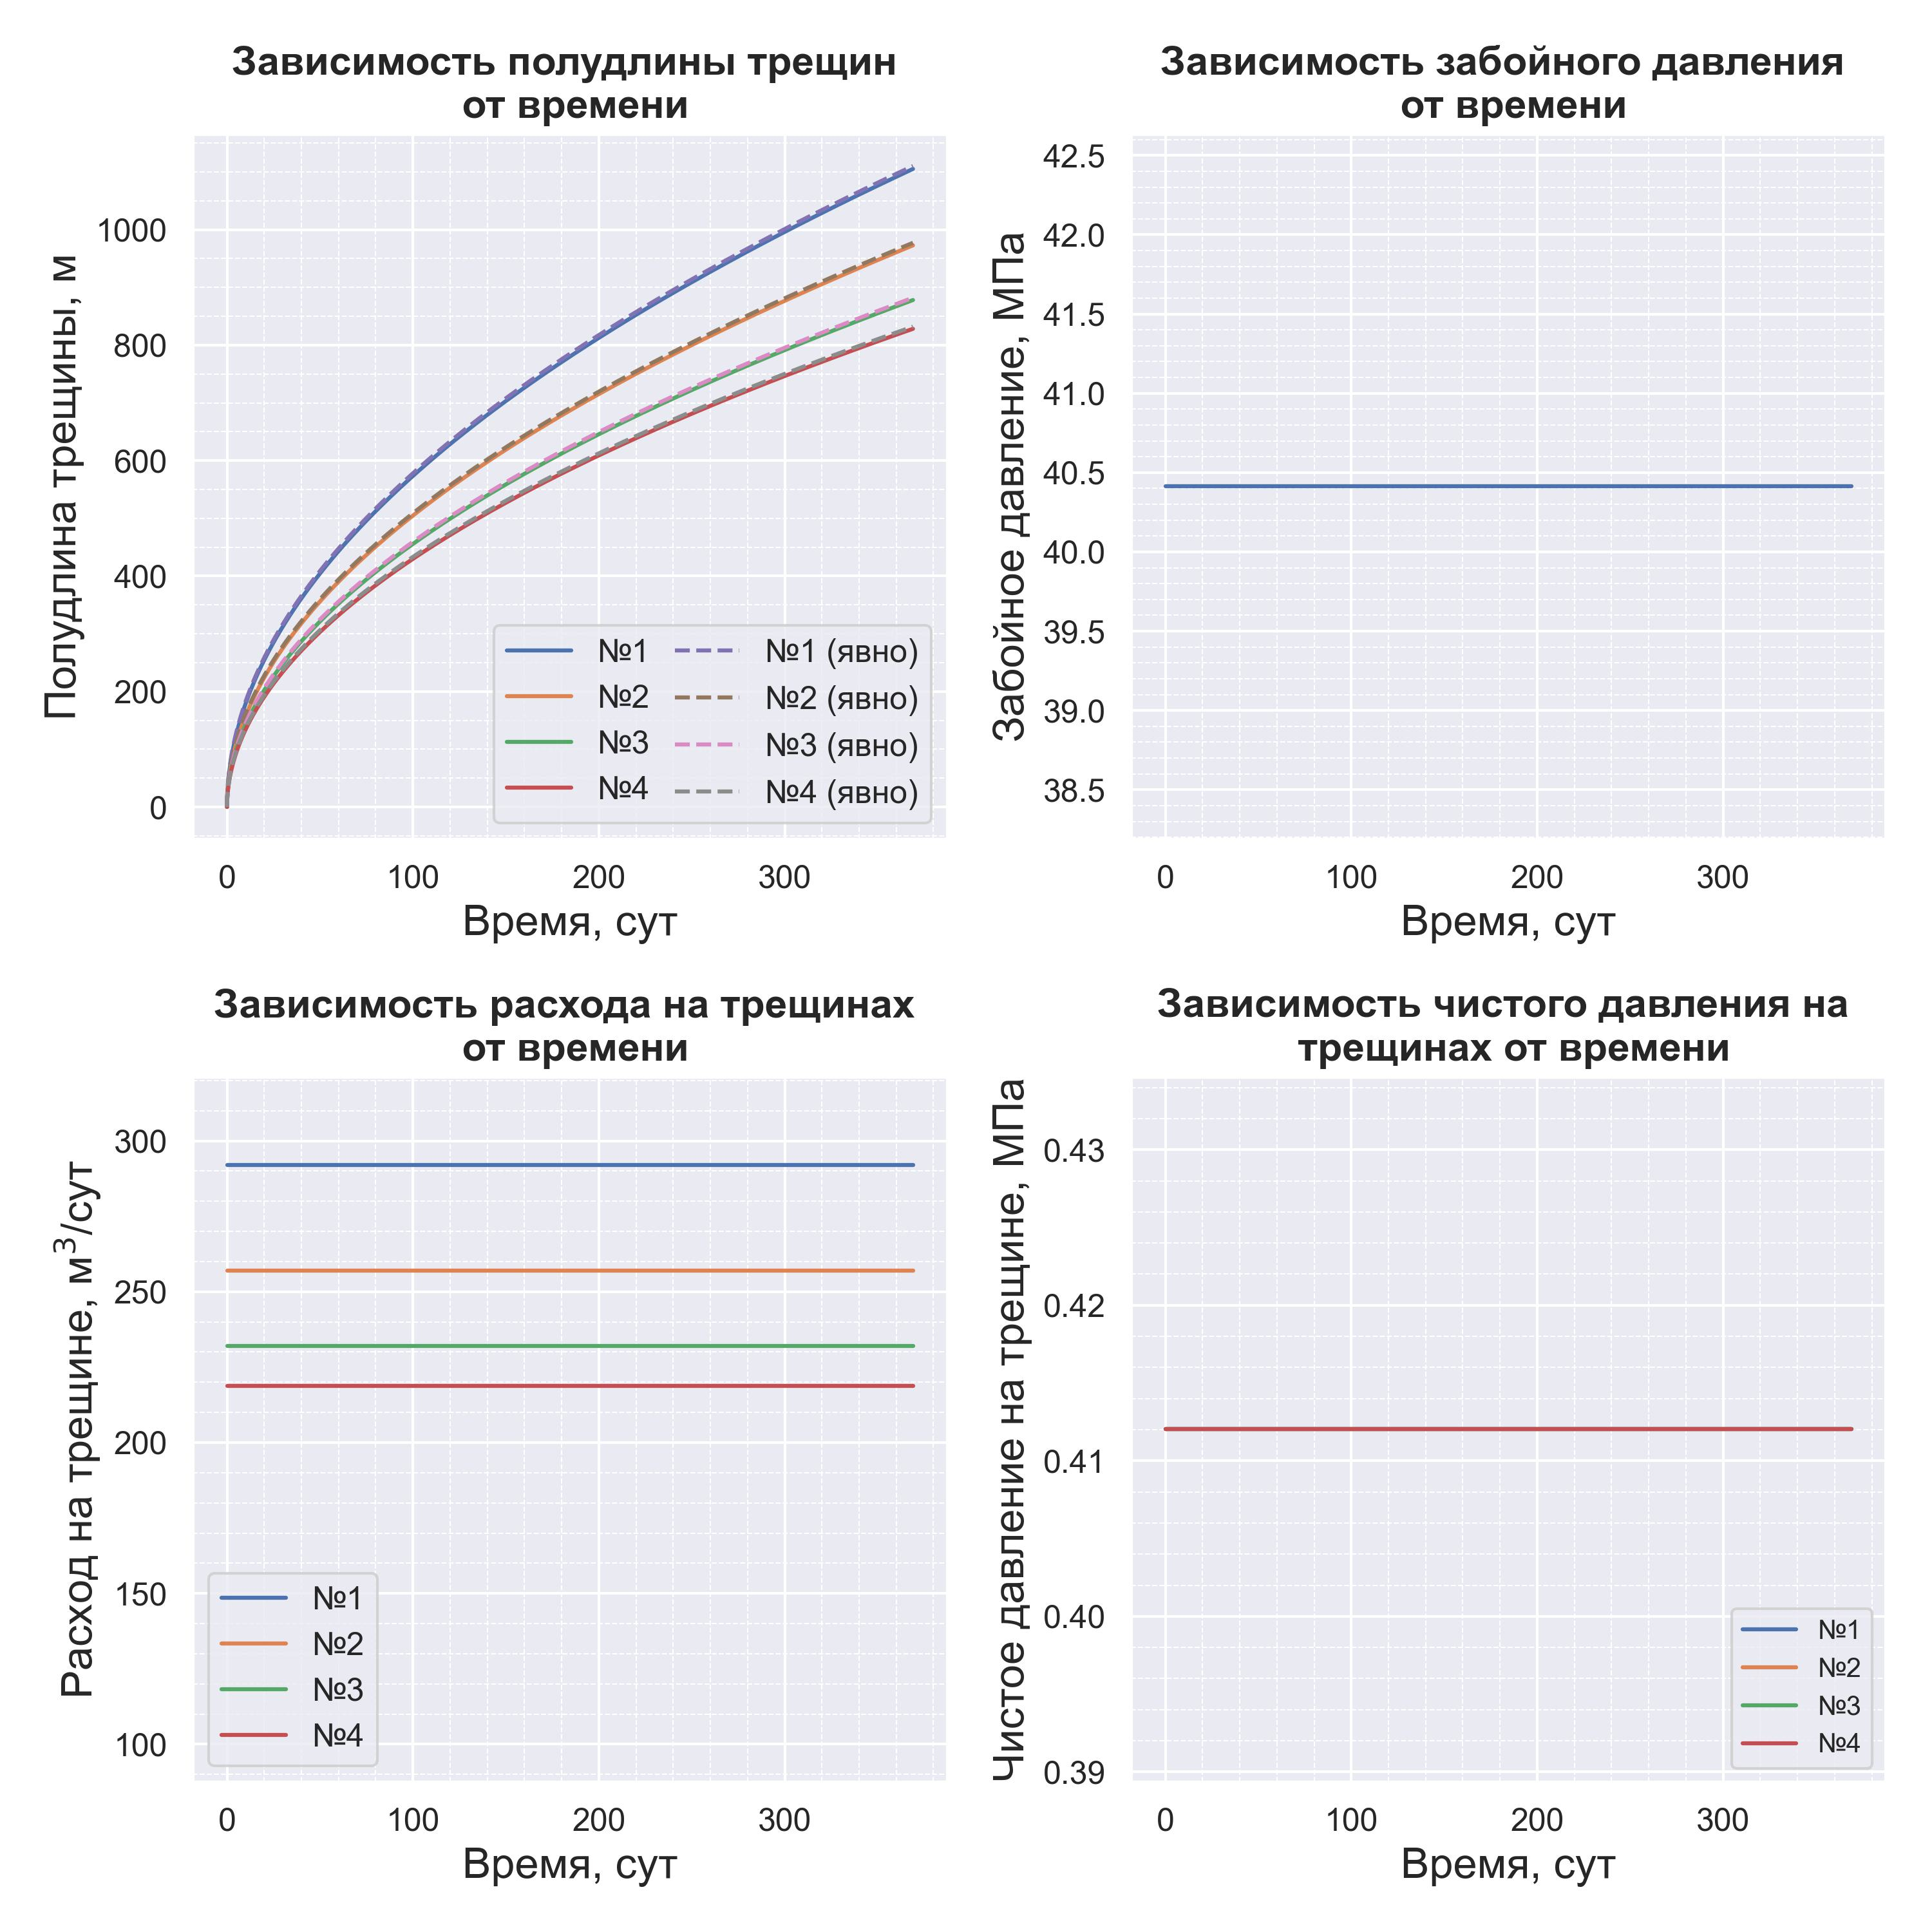
\includegraphics[width=\linewidth]{images/myimage1.jpg}
\caption{Результаты моделирования перераспределения потоков и роста трещин автоГРП в случае одномерных утечек Картера при выбранных значениях входных параметров}
\label{fig:myimage1}
\end{figure}

Видим, что расходы на трещинах постоянны и длина трещин растёт согласно первой формуле Кёнинга \eqref{Koning_first}.
Чистое давление в трещинах постоянно, так как предполагается, что все трещины распространяются и давление в них равно давлению распространения трещин PKN.
Забойное давление также постоянно, так как расходы (и соответственно перепады давления на трение в трубе и на перфорациях) не меняются со временем.

Такой же эксперимент при выбранных значениях параметров (см. табл. \ref{tab:input-parameters-for-fractures-growth}) проведён в случае двумерных радиальных утечек жидкости из трещины в пласт.
Результаты представлены на рис. \ref{fig:myimage2}.

\begin{figure}[H] 
\center
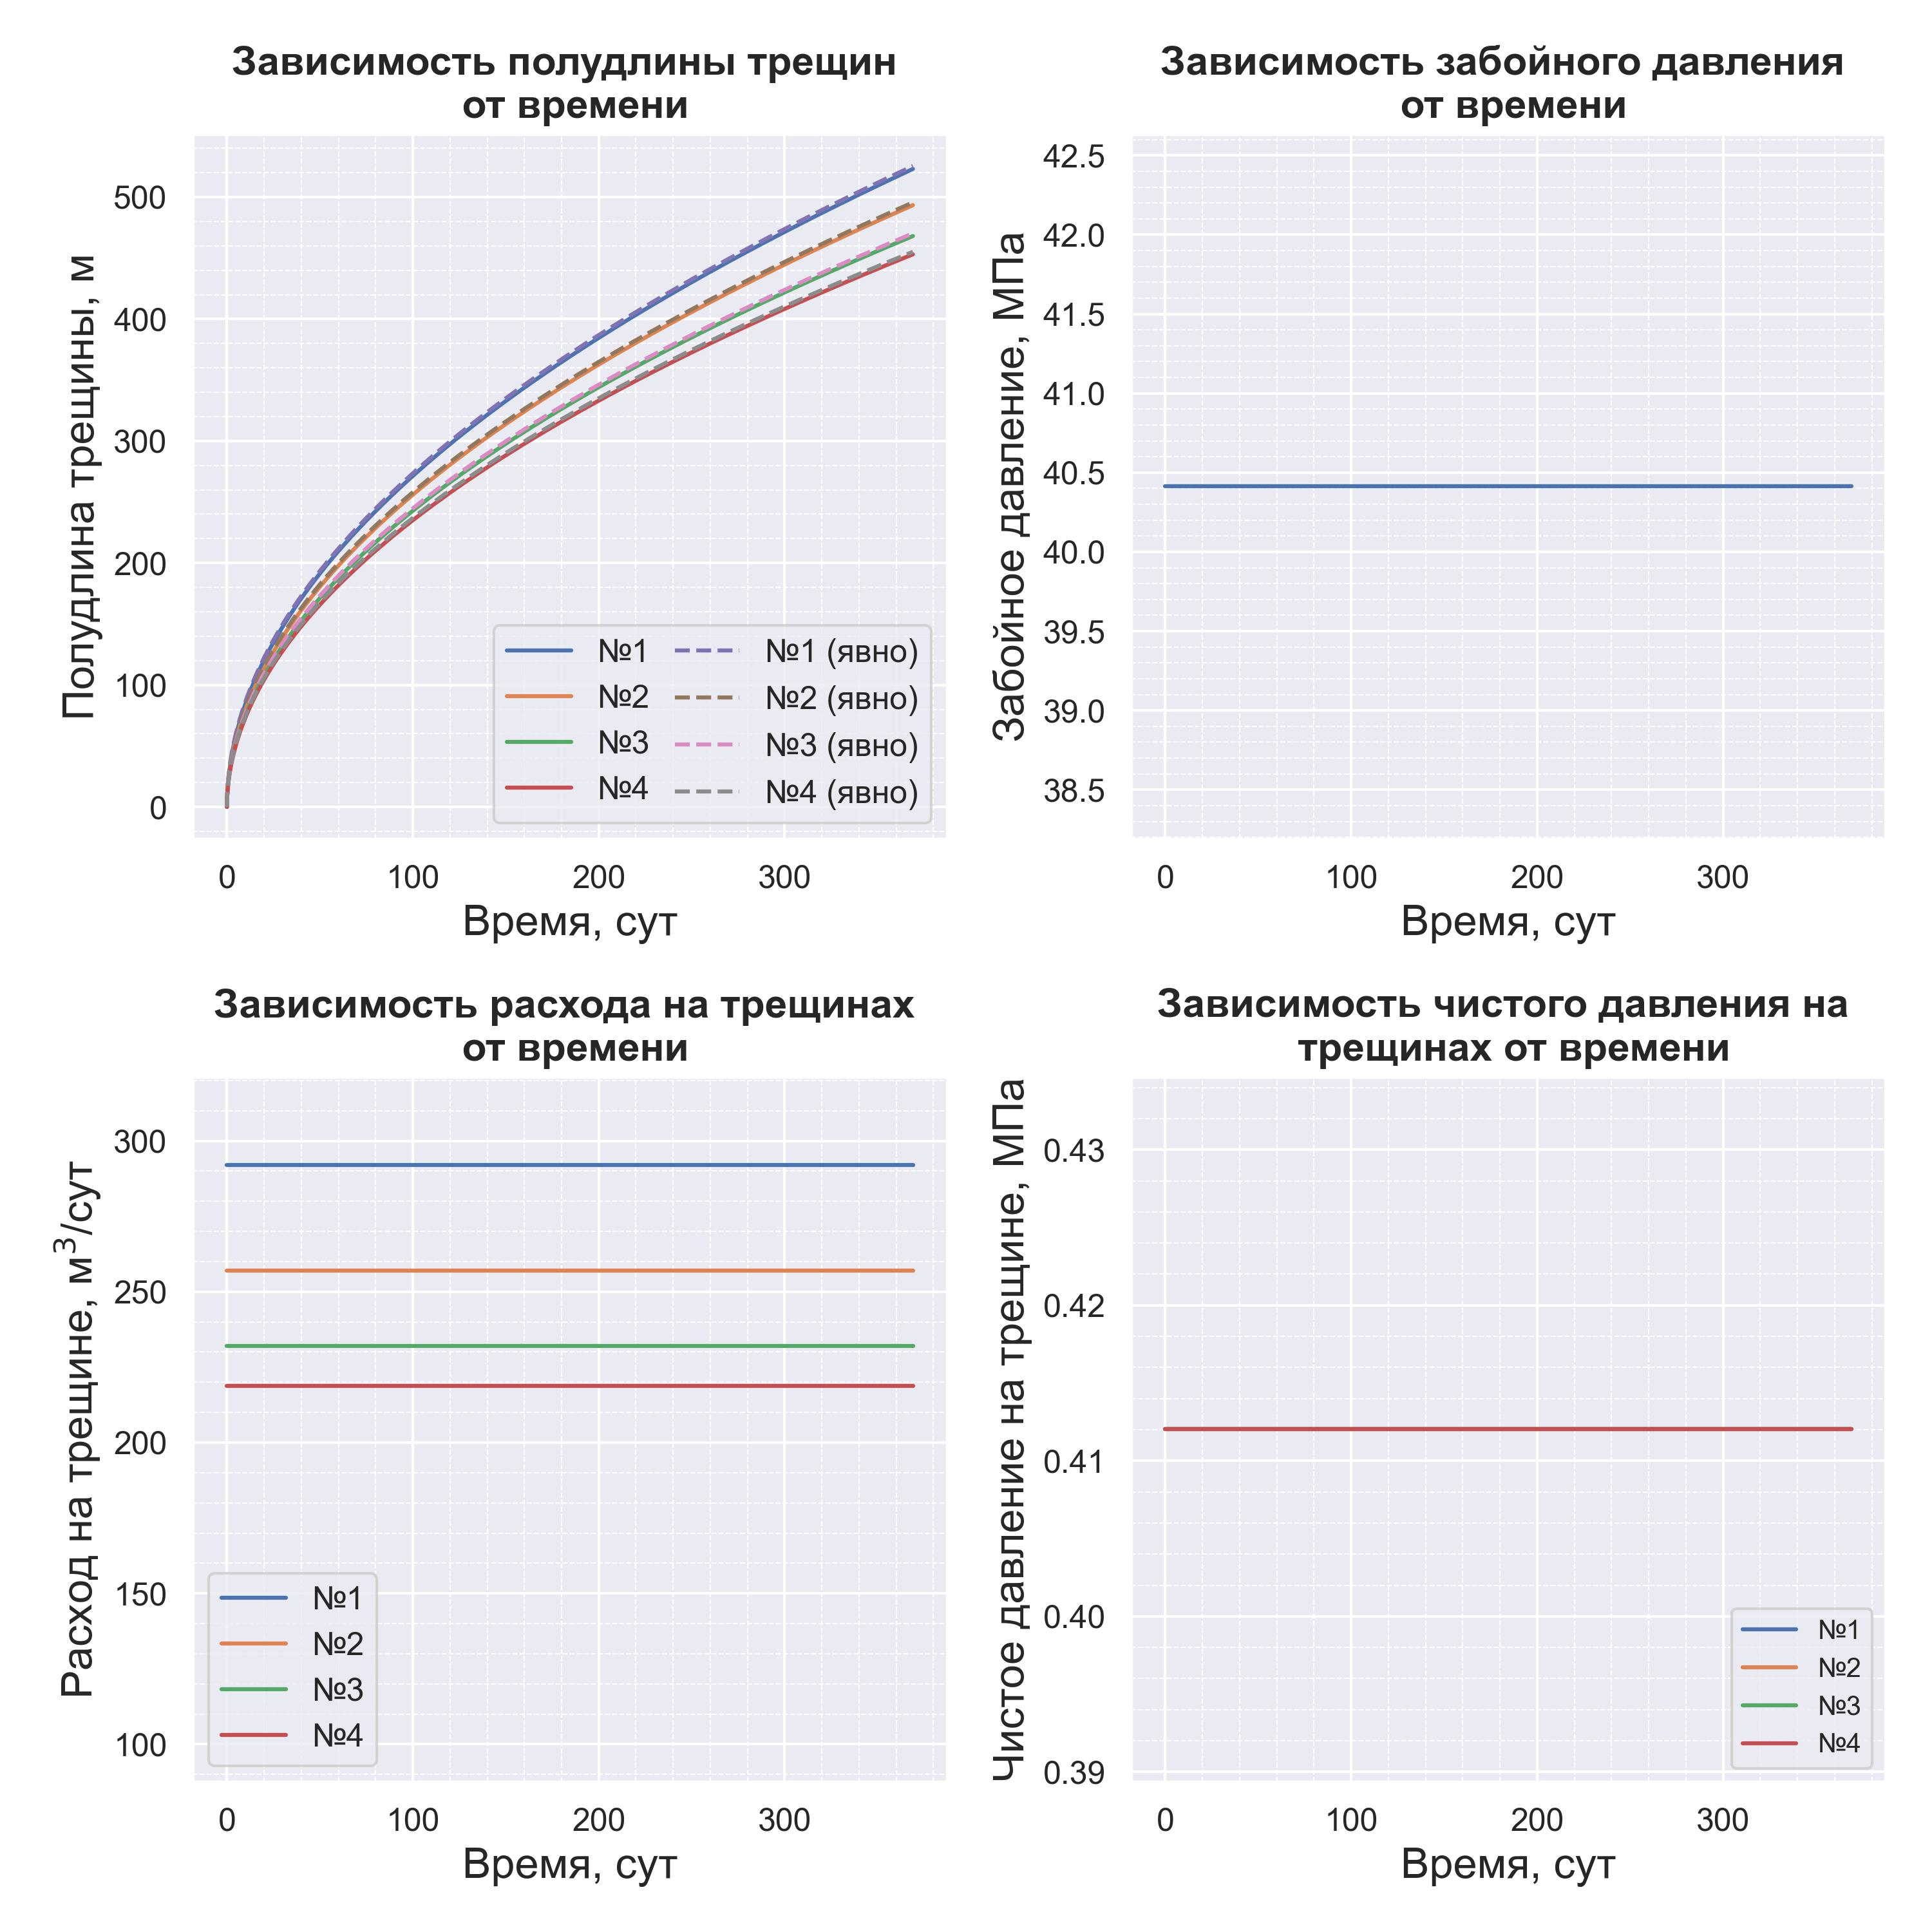
\includegraphics[width=.95\linewidth]{images/myimage2.jpg}
\caption{Результаты моделирования перераспределения потоков и роста трещин автоГРП в случае двумерных радиальных утечек жидкости из трещины при выбранных значениях входных параметров} 
\label{fig:myimage2}
\end{figure}

В этом случае (см. рис. \ref{fig:myimage2}) трещины растут по второй формуле Кёнинга \eqref{Koning_second} и их длина в каждый момент времени меньше, чем длина, полученная в случае одномерных утечек Картера, что согласуется с результатами работы \cite{hagoort}.

Таким образом, предположение одномерности утечек по Картеру \cite{karter_book} может завышать оценку для длины растущих трещин автоГРП.

При ухудшении качества перфораций на второй, третьей и четвёртой трещинах наблюдается интересная картина (см. рис. \ref{fig:myimage9} и рис. \ref{fig:myimage10}) стремительного роста первой трещины, на которой качество перфораций не изменяется.
Особенно сильно этот эффект заметен в случае одномерных утечек Картера.

Диаметр перфораций на второй, третьей и четвёртой трещинах изменялся по следующим формулам:
\beq
d_{p,2}(t)=0.02\text{ м}-0.015\text{ м}\cdot\left(\frac{t}{365\text{ сут}}\right)
\eeq
\beq
d_{p,3}(t)=0.02\text{ м}-0.010\text{ м}\cdot\left(\frac{t}{365\text{ сут}}\right)
\eeq
\beq
d_{p,4}(t)=0.02\text{ м}-0.005\text{ м}\cdot\left(\frac{t}{365\text{ сут}}\right)
\eeq

\begin{figure}[H] 
\center
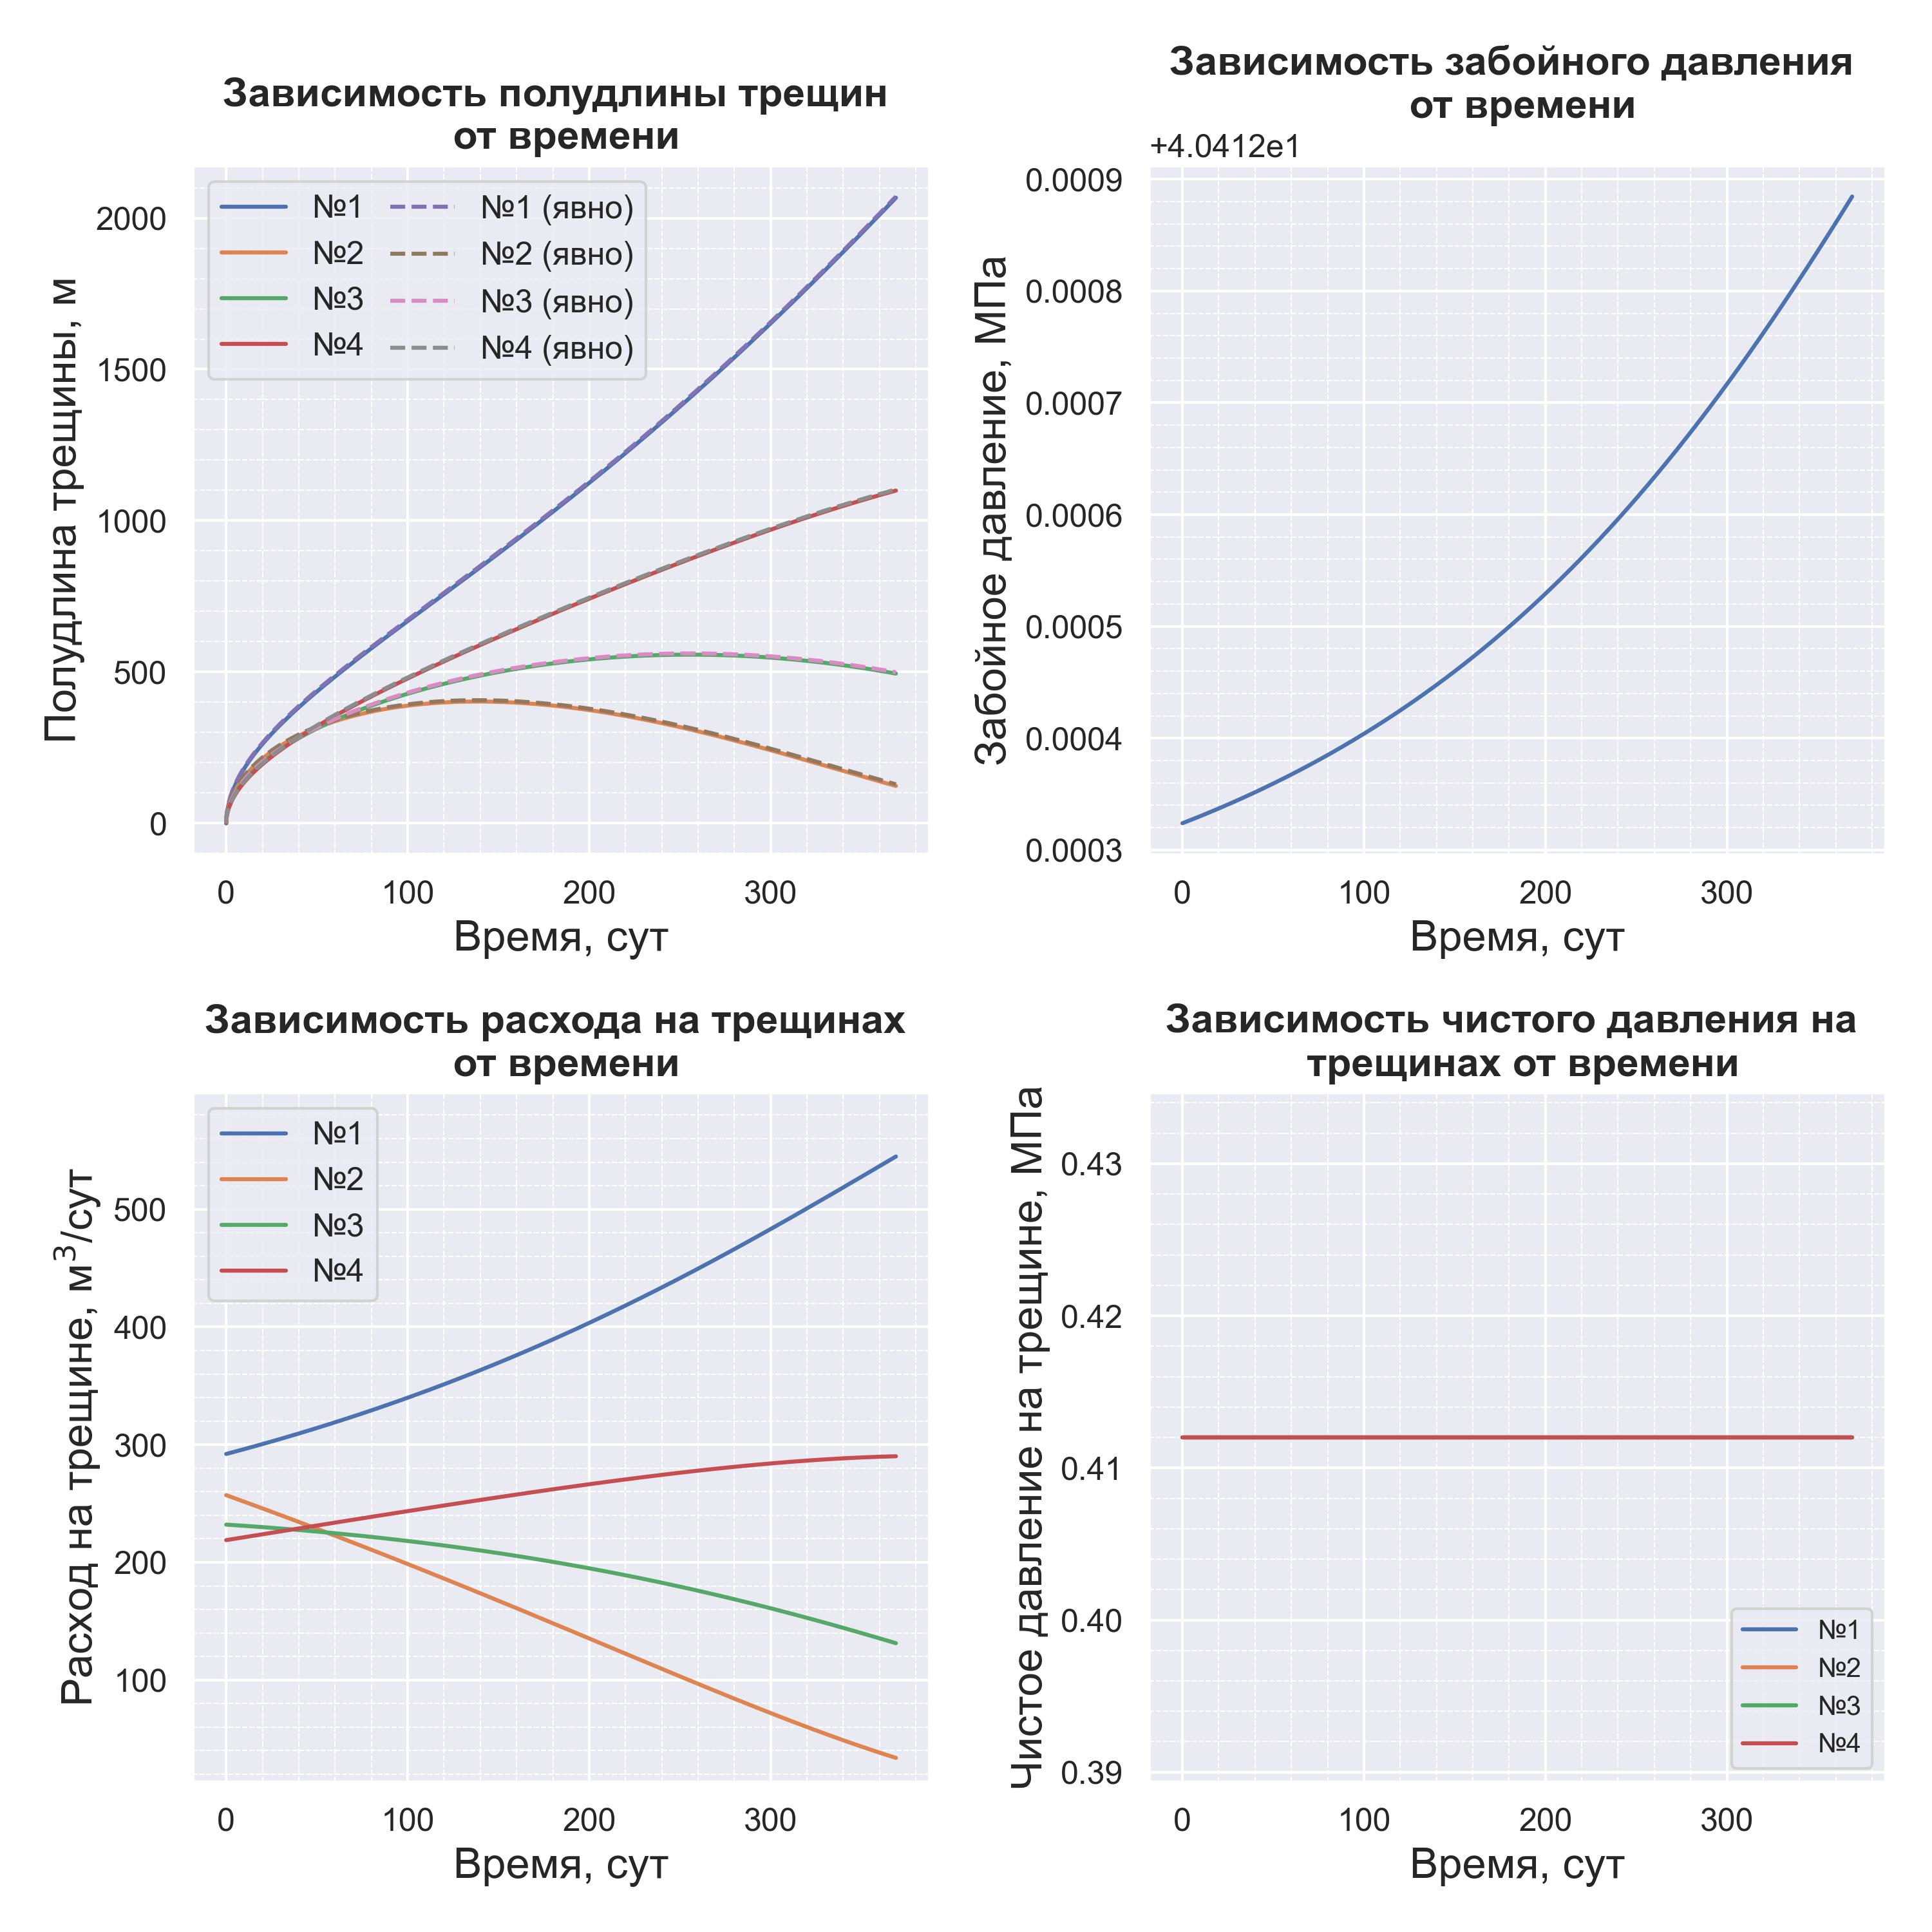
\includegraphics[width=0.9\linewidth]{images/myimage9.jpg}
\caption{Результаты моделирования перераспределения потоков и роста трещин автоГРП при уменьшении диаметра перфораций на второй, третьей и четвёртой трещинах -- режим утечек Картера}
\label{fig:myimage9}
\end{figure}


\begin{figure}[H] 
\center
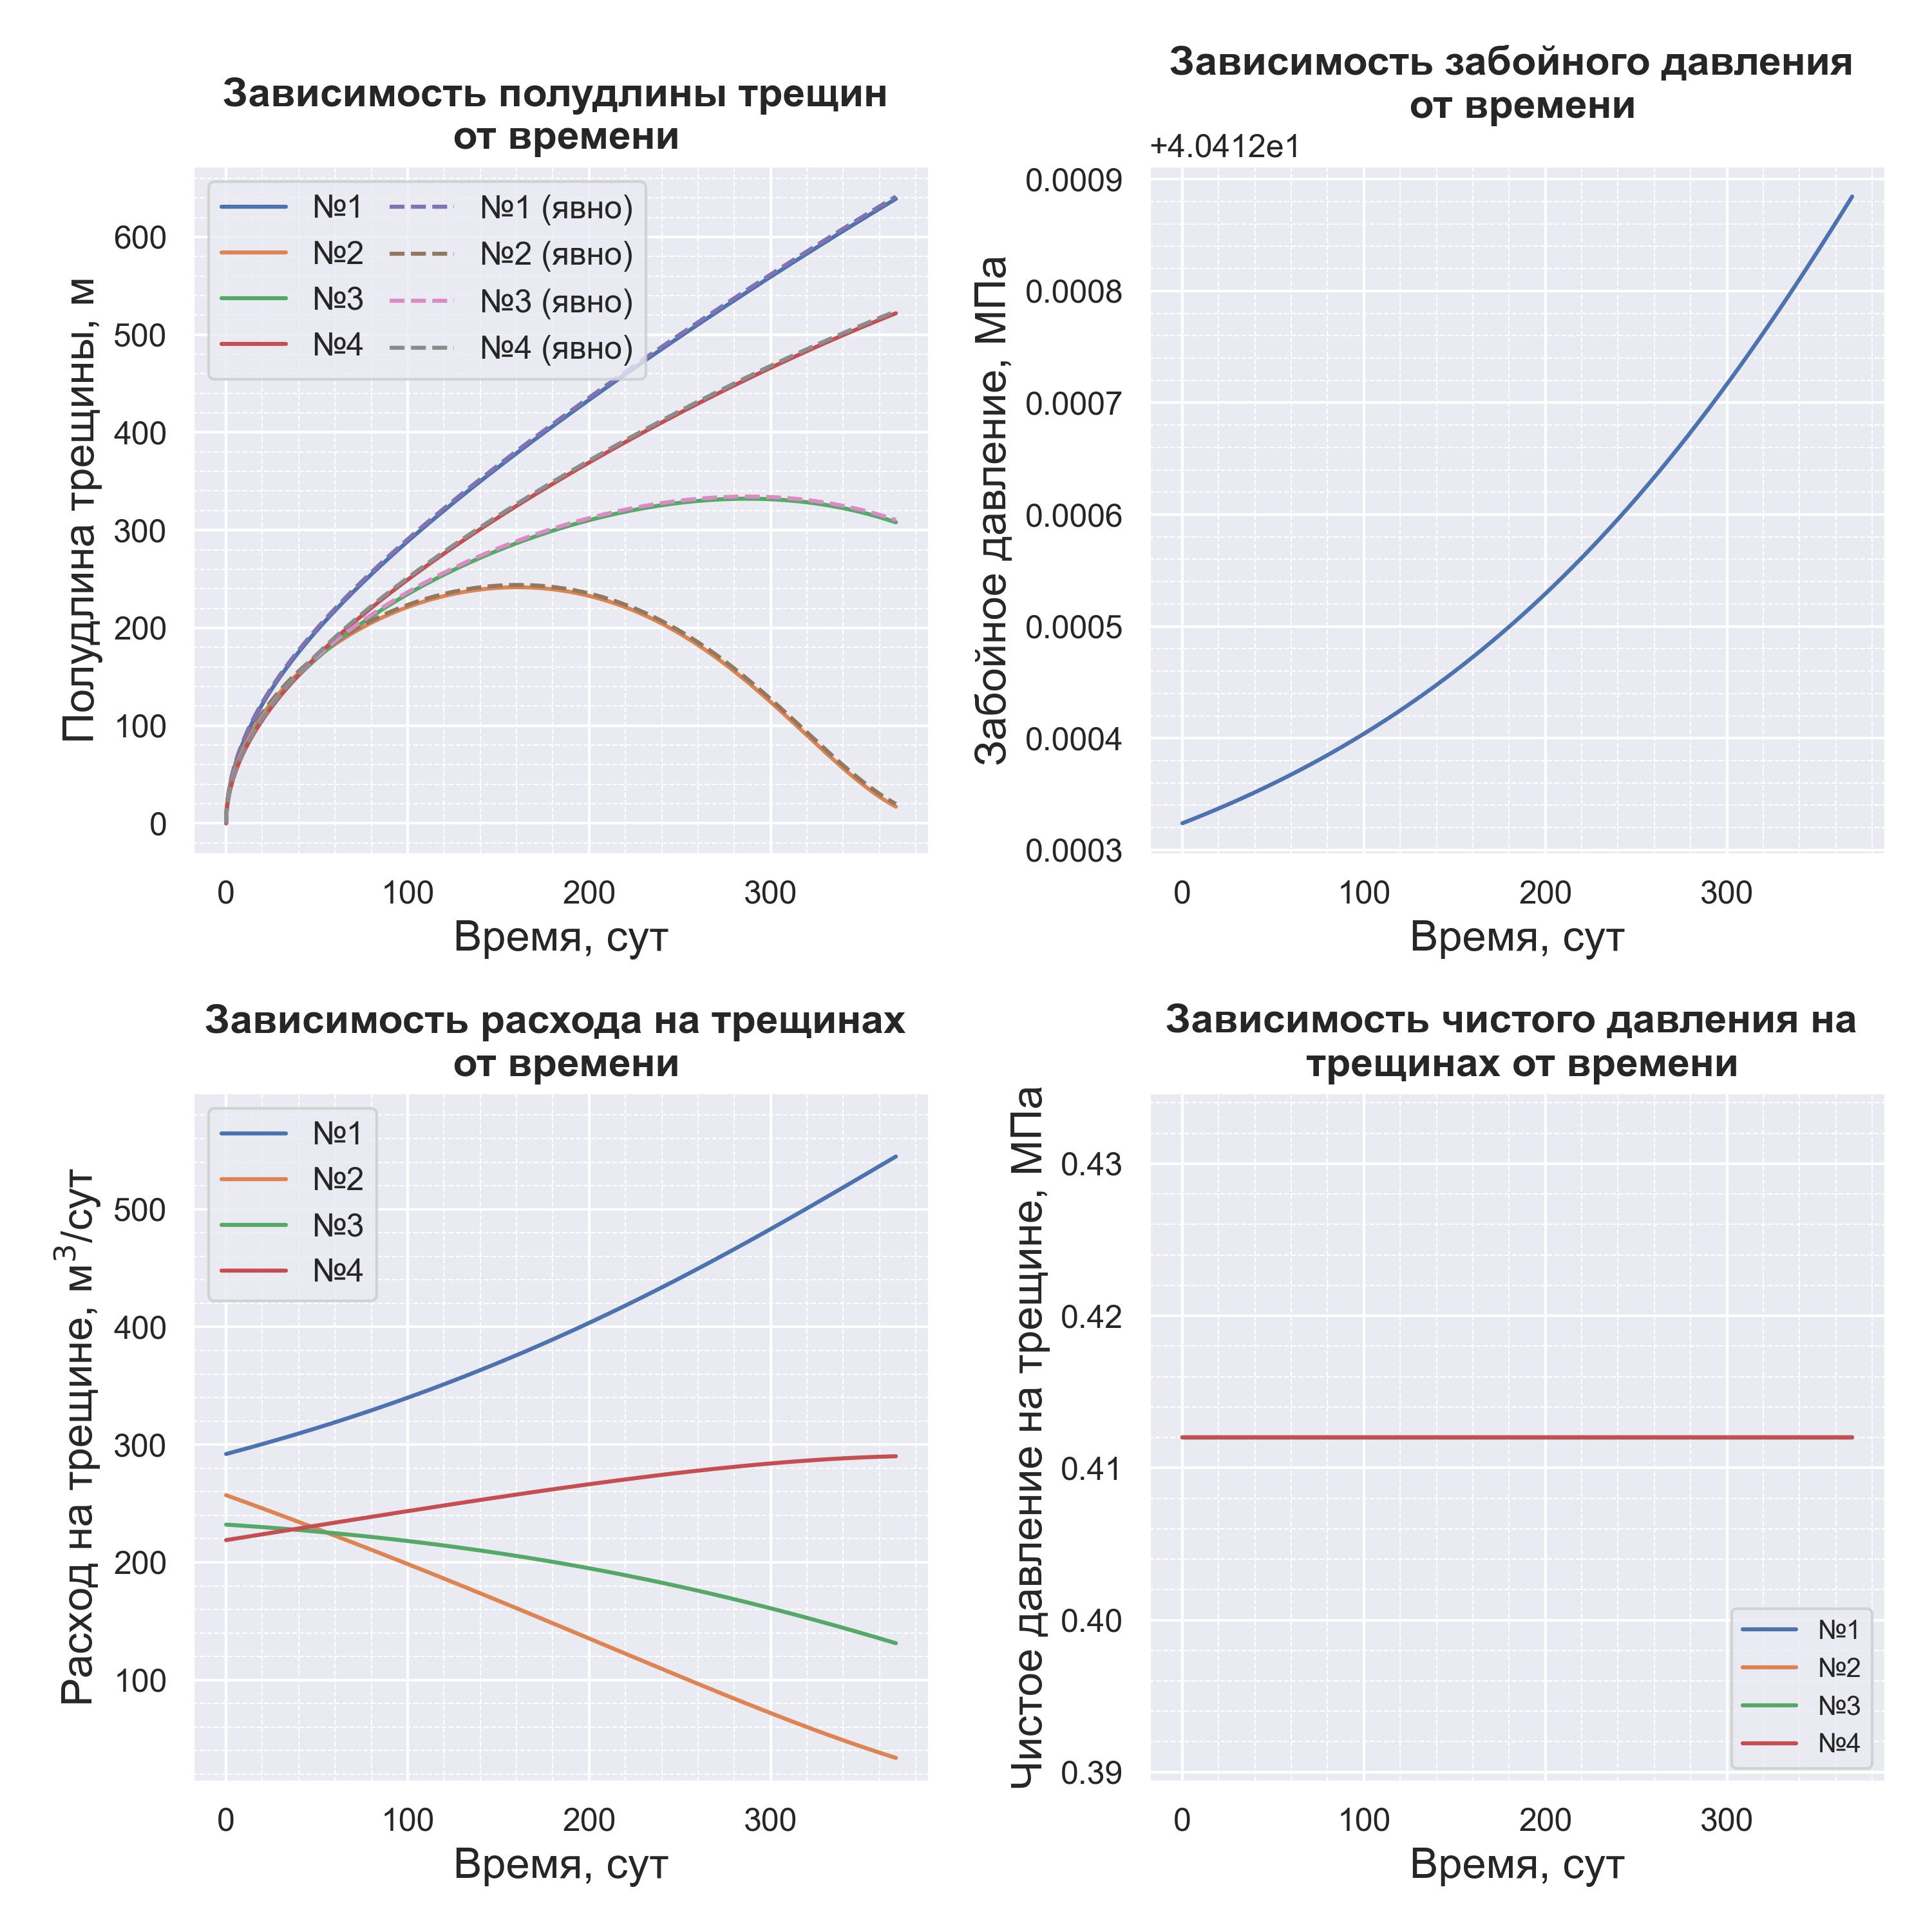
\includegraphics[width=\linewidth]{images/myimage10.jpg}
\caption{Результаты моделирования перераспределения потоков и роста трещин автоГРП при уменьшении диаметра перфораций на второй, третьей и четвёртой трещинах -- двумерный радиальный режим утечек жидкости из трещины в пласт}
\label{fig:myimage10}
\end{figure}

Далее проведён эксперимент при уменьшении горизонтальных напряжений пласта со временем (за счёт термоупругого воздействия -- например, в пласт закачивается холодная вода).
Результаты представлены на рис. \ref{fig:myimage11} и \ref{fig:myimage12}.
Минимальное горизонтальное напряжения в пласте в этом эксперименте изменялось по формуле:
\beq
\sigma_{\text{min}}(t)=40\text{ МПа}-5\text{ МПа}\cdot\left(\frac{t}{365\text{ сут}}\right)
\eeq

\begin{figure}[H] 
\center
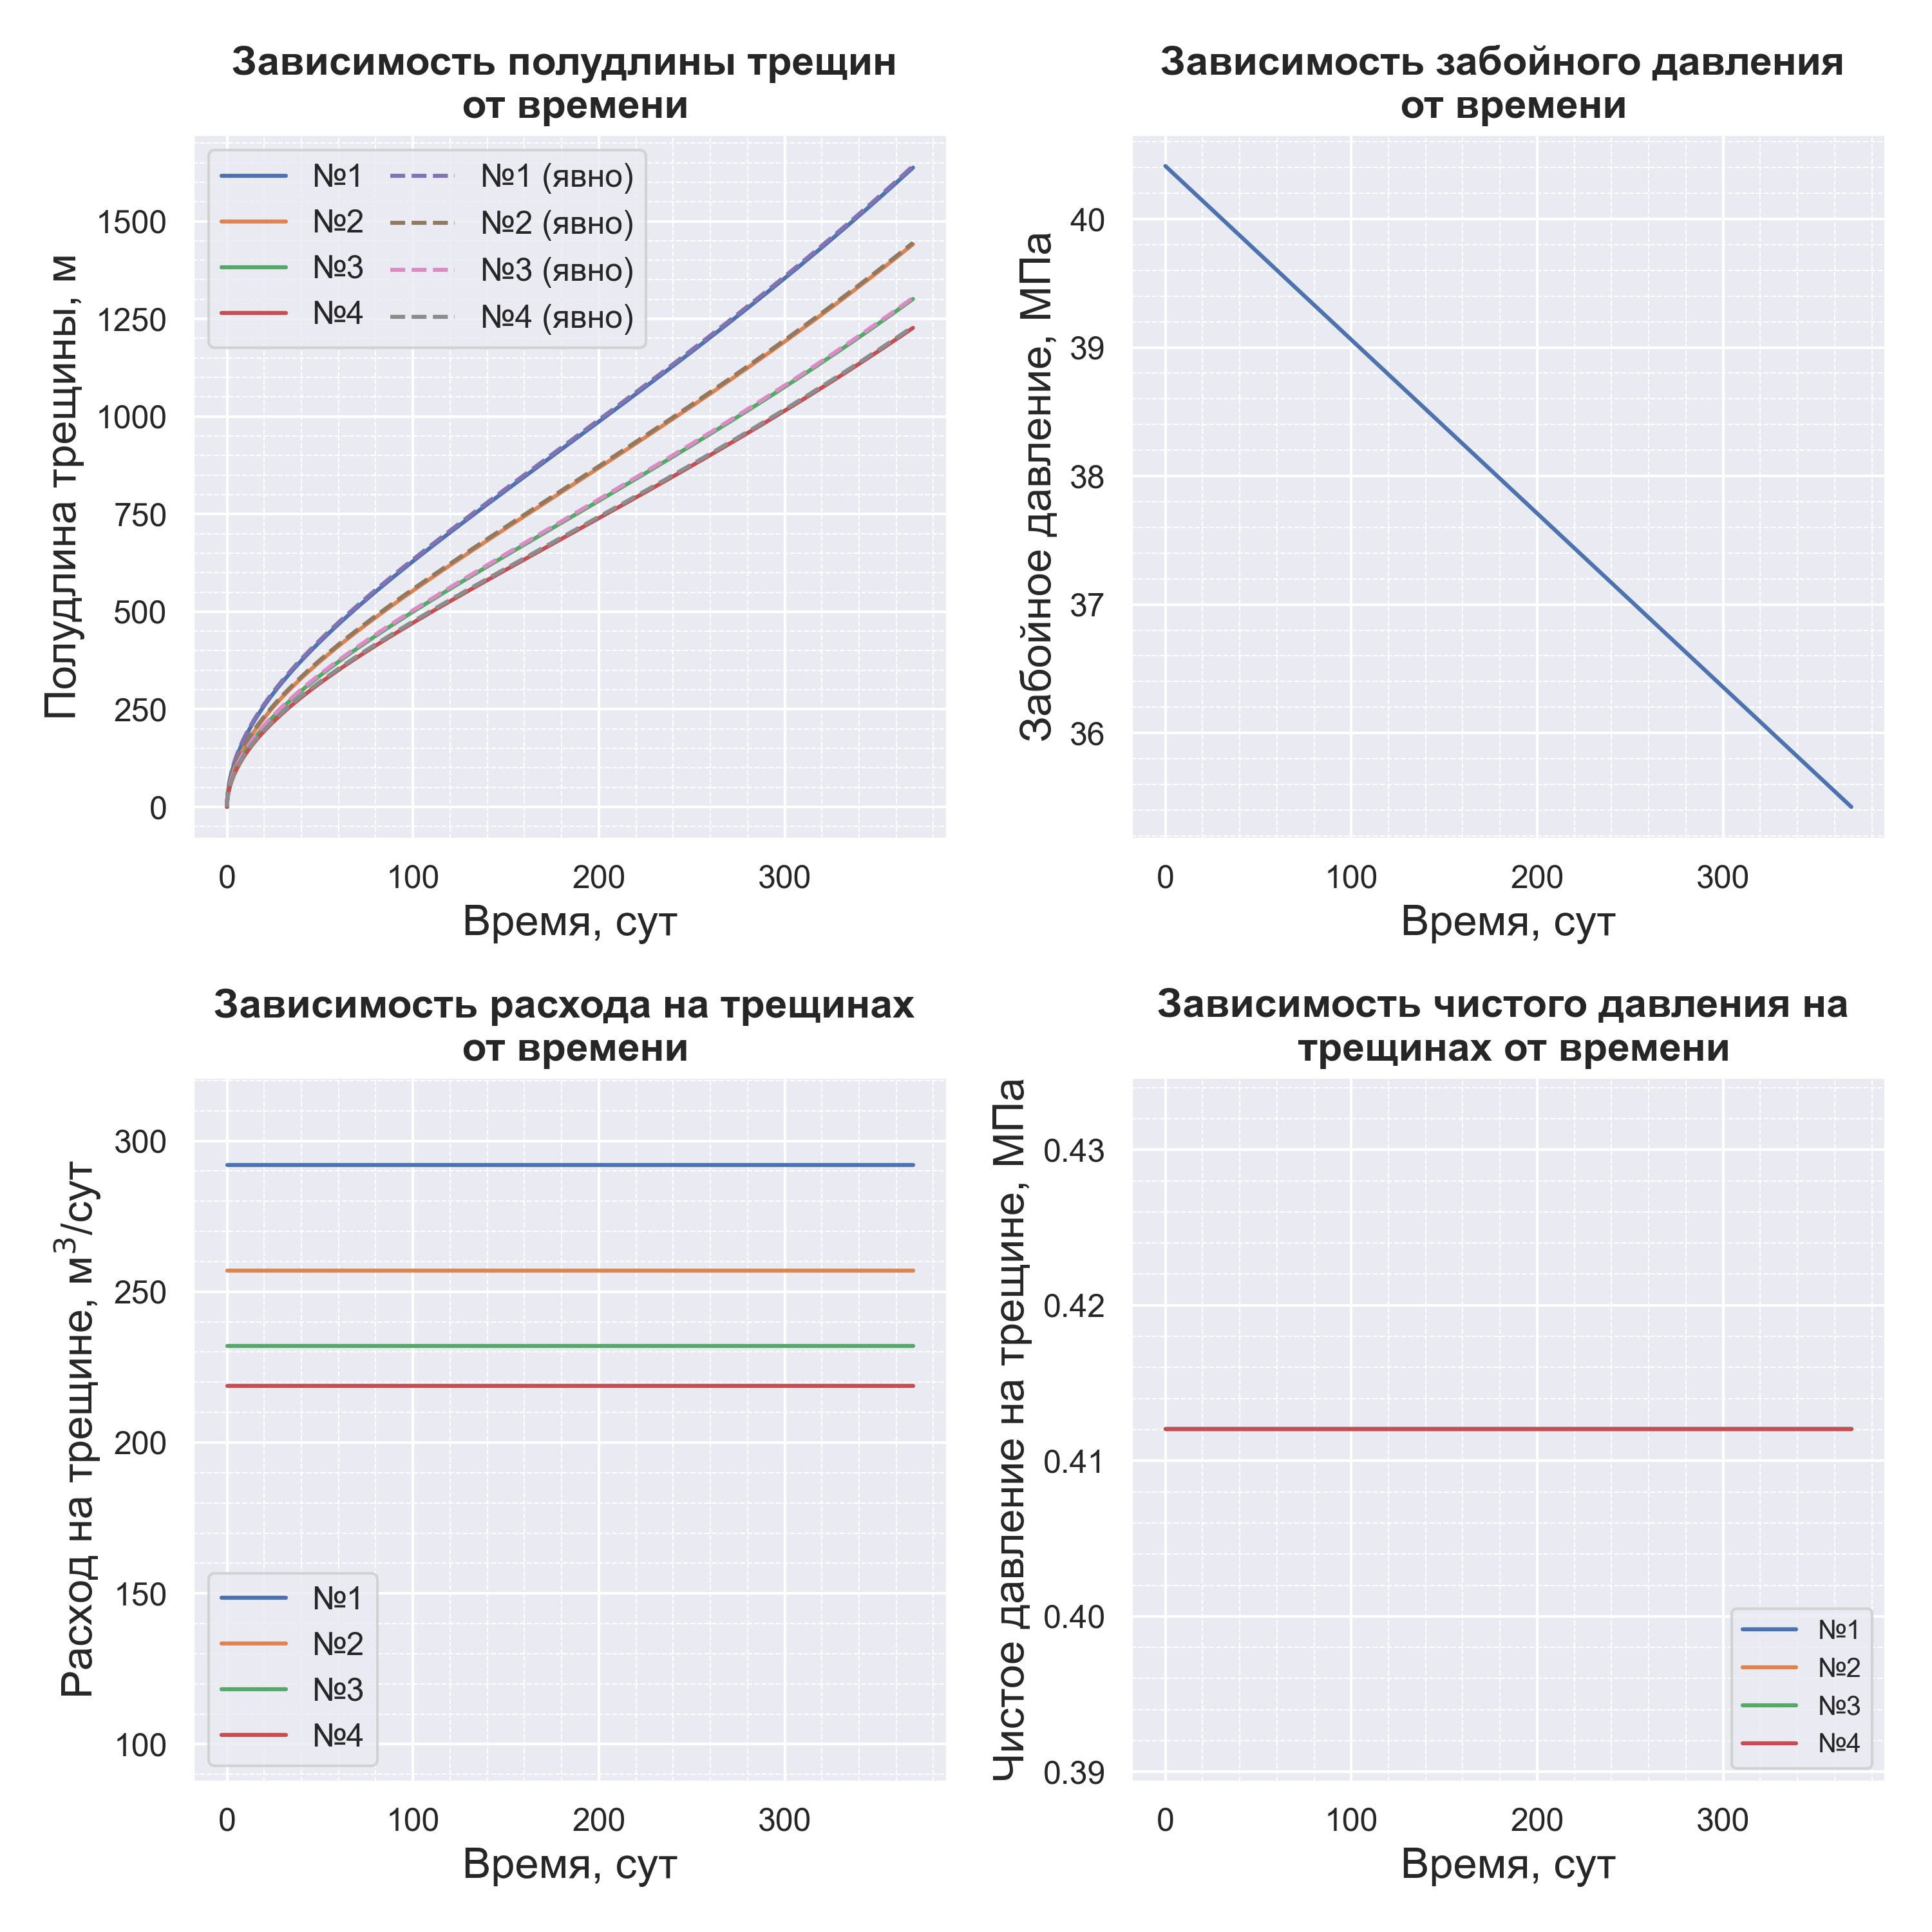
\includegraphics[width=\linewidth]{images/myimage11.jpg}
\caption{Результаты моделирования перераспределения потоков и роста трещин автоГРП при термоупругом воздействии (уменьшении горизонтальных напряжений в пласте) -- режим утечек Картера}
\label{fig:myimage11}
\end{figure}

Из рис. \ref{fig:myimage11} и рис. \ref{fig:myimage12} видим, что термоупругое уменьшение горизонтальных напряжений пласта  приводит к более длинным трещинам (по сравнению с базовым сценарием рис. \ref{fig:myimage1} и \ref{fig:myimage2}), что согласуется с результатами работы \cite{perkins_gonzalez}.

\begin{figure}[H] 
\center
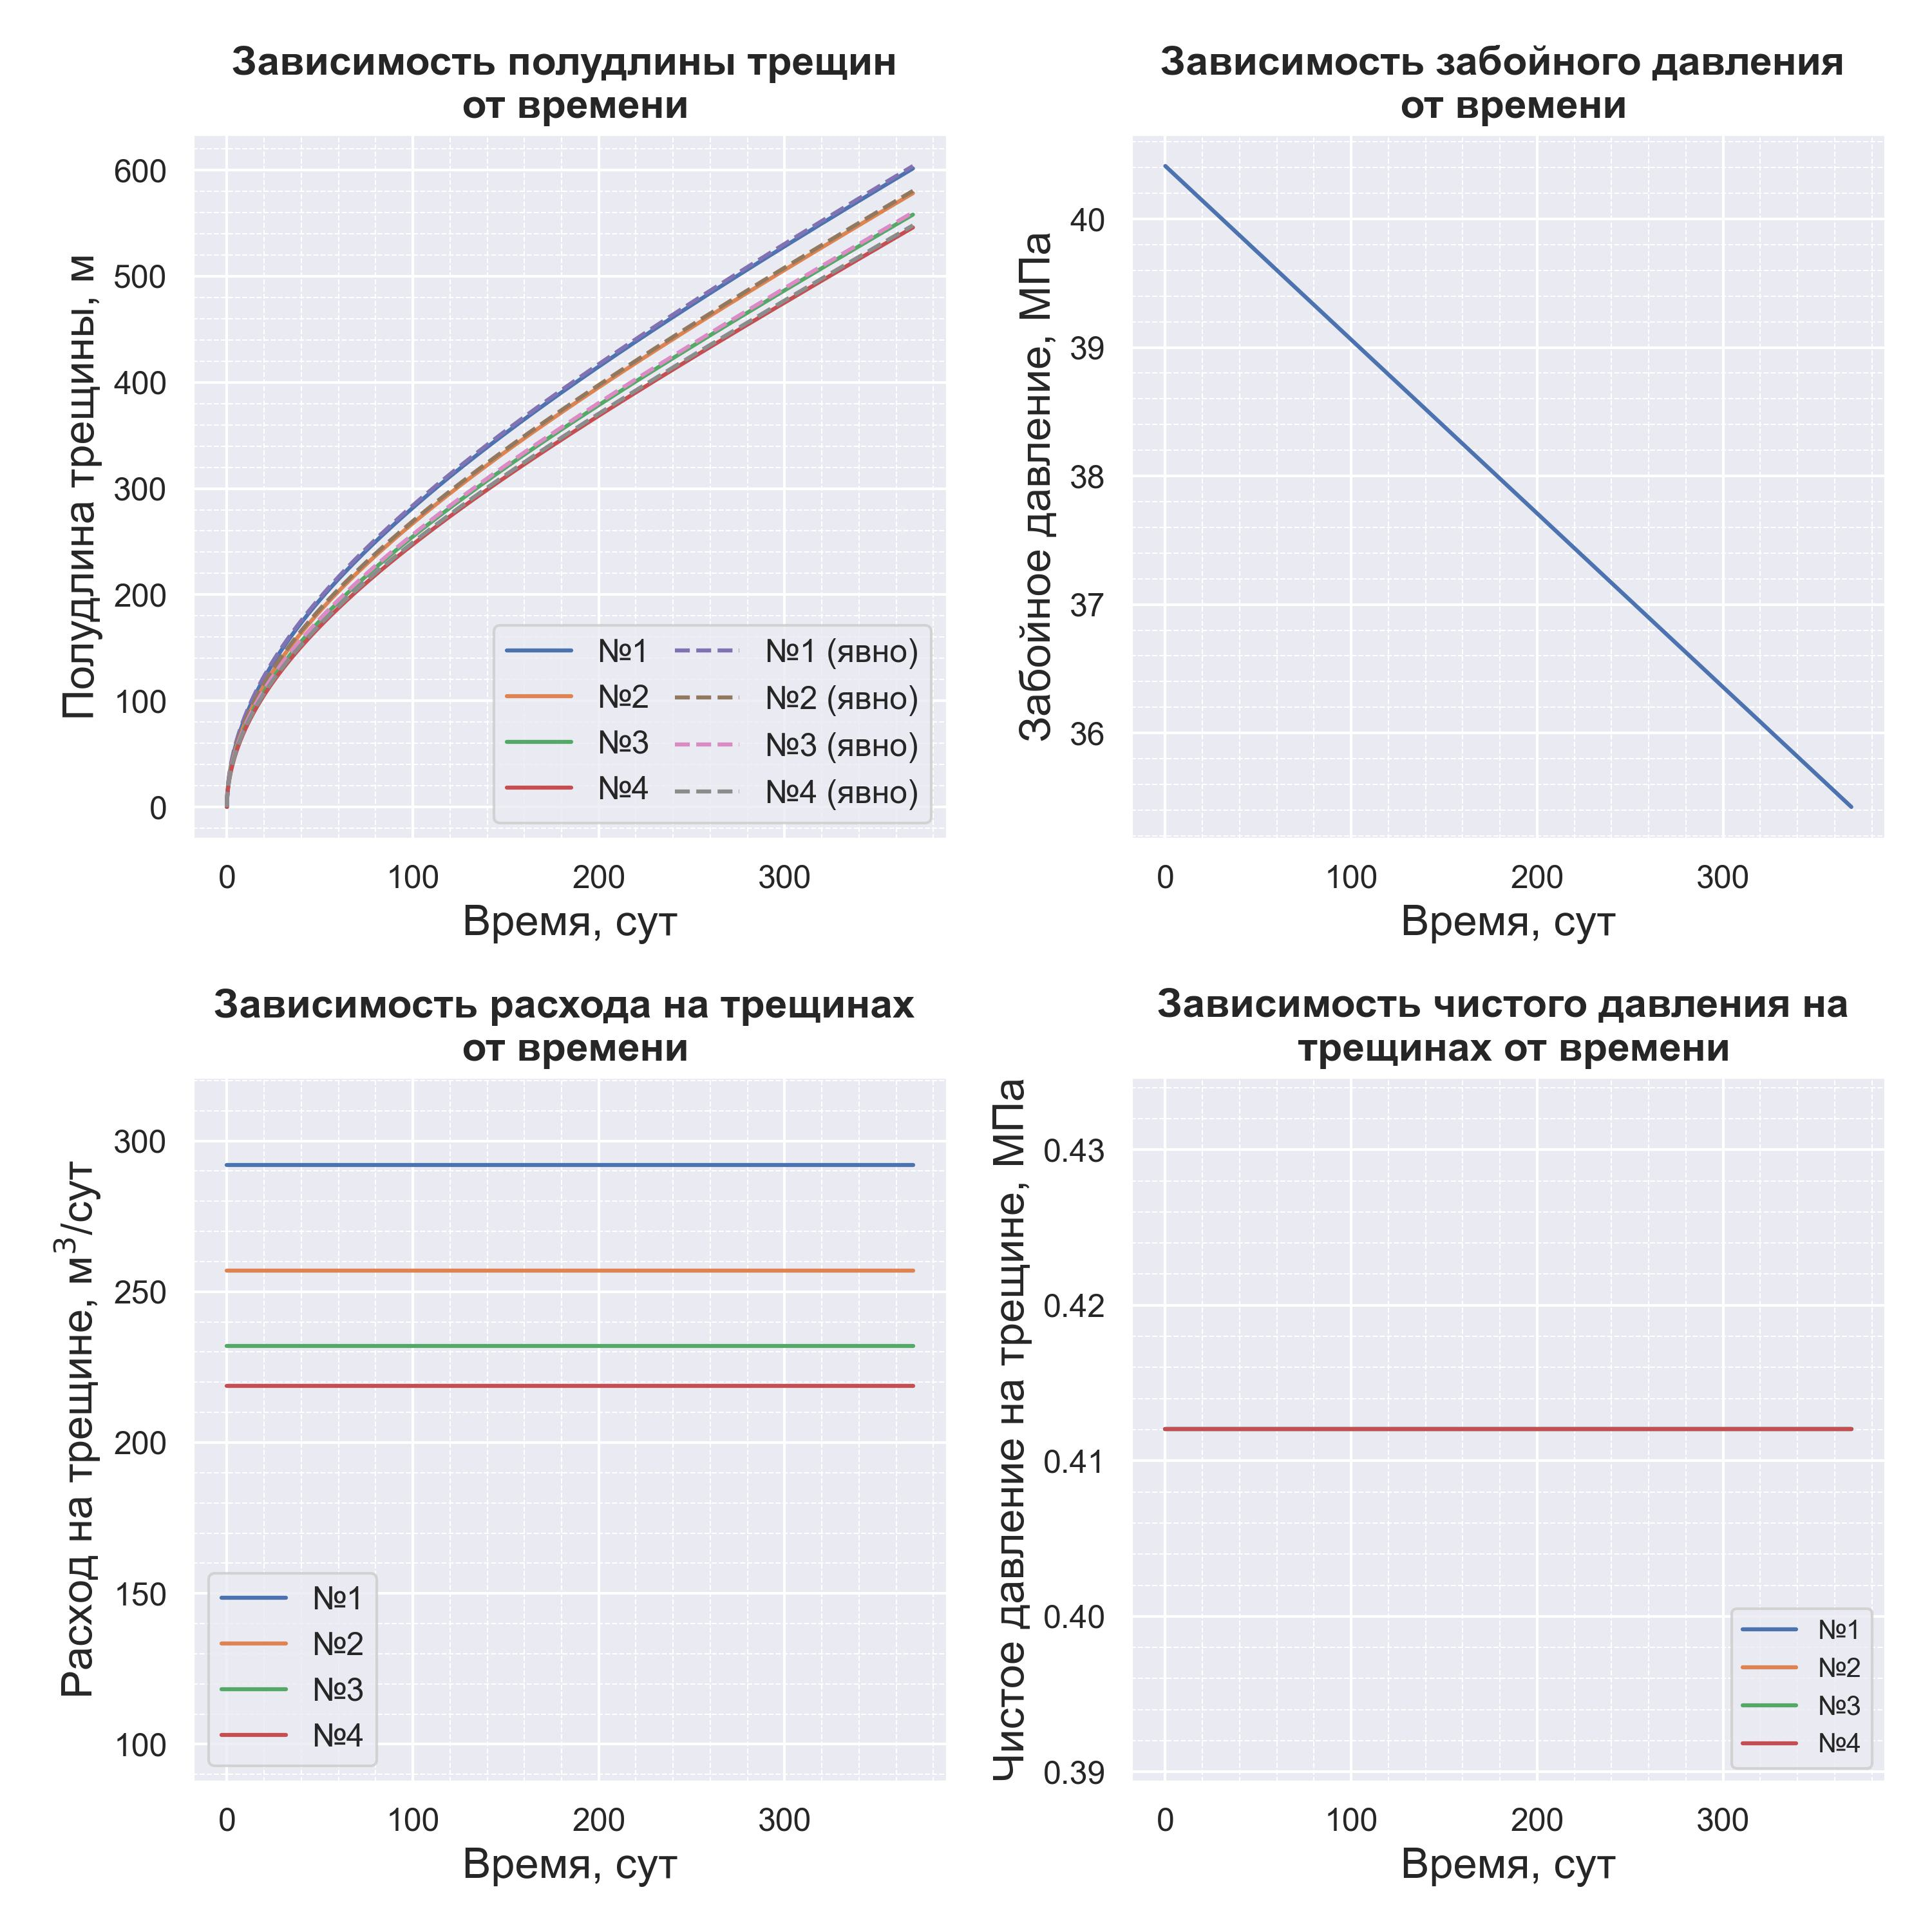
\includegraphics[width=\linewidth]{images/myimage12.jpg}
\caption{Результаты моделирования перераспределения потоков и роста трещин автоГРП при термоупругом воздействии (уменьшении горизонтальных напряжений в пласте) -- двумерный радиальный режим утечек жидкости из трещины в пласт}
\label{fig:myimage12}
\end{figure}

